\documentclass[aspectratio=169]{beamer}
\usepackage{pgfpages}
\setbeamertemplate{note page}[plain]

%enable notes
%\setbeameroption{show notes on second screen=right}
\usepackage[T1]{fontenc}
\usepackage[utf8]{inputenc}
\usepackage{lmodern}
\usepackage[french]{babel}
\usepackage{hyperref}
\usepackage{graphicx}
\usepackage{makecell}
\usepackage{xcolor}
\usepackage{colortbl}
\usepackage[flushleft]{threeparttable}
\setbeamertemplate{note page}{\pagecolor{yellow!5}\insertnote}\usepackage{palatino}

\graphicspath{ {./img/} }

%\newcommand{\TODO}{TODO:}
\newcommand*{\rot}{\rotatebox{90}}


% \title{Bacula\\~\\AIT --- Présentation}

\title{
    AIT --- Présentation \\~\\
    \centering
\includegraphics [height=20mm] {logo_bacula.png} 
}
% \titlegraphic{
\includegraphics [height=.2\textheight] {logo_bacula.png}}
\author{Gwendoline Dössegger, Noémie Plancherel, Gaby Roch, Cassandre Wojciechowski}
\author{Cassandre Wojciechowski \\ Gwendoline Dössegger \\ Noémie Plancherel \\ Gaby Roch}
\hypersetup{pdfauthor={G. Dössegger, N. Plancherel, G. Roch, C. Wojciechowski}}
\date{8 novembre 2021}

\begin{document}

\begin{frame}
  \titlepage
\end{frame}

\begin{frame}{Bacula -- Présentation générale}
 \begin{itemize}
  \item Logiciel de sauvegarde multi-platform créé en 2000 par Kern Sibbald
  \item Première version 2002
  \item Dernière version 11.0.5, juin 2021
  \item Open source / private source
 \end{itemize}
\note{Bacula est un logiciel de sauvegarde multi-platforme. Il a été développé à partir de l'année 2000 par Kern Sibbald et sa première version a été publiée deux ans plus tard, c'est-à-dire en 2002. 
\\~\\
Le logiciel est continuellement maintenu, documenté et mis à jour. Pour vous donnez une idée, la dernière release est sortie en juin de cette année. 
\\~\\
Bacula possède une version community qui est Open Source. Ses différents composants peuvent tourner sur des systèmes d'exploitation gratuit (par ex linux) ce qui ne nécessite pas l'achat de licences supplémentaires pour tester le logiciel.
\\~\\
Il existe une version entreprise avec plus de fonctionnalités mais cette fois-ci payante que l'on vous présentera par la suite.}
\end{frame}

\begin{frame}{Architecture}
  \begin{center}
    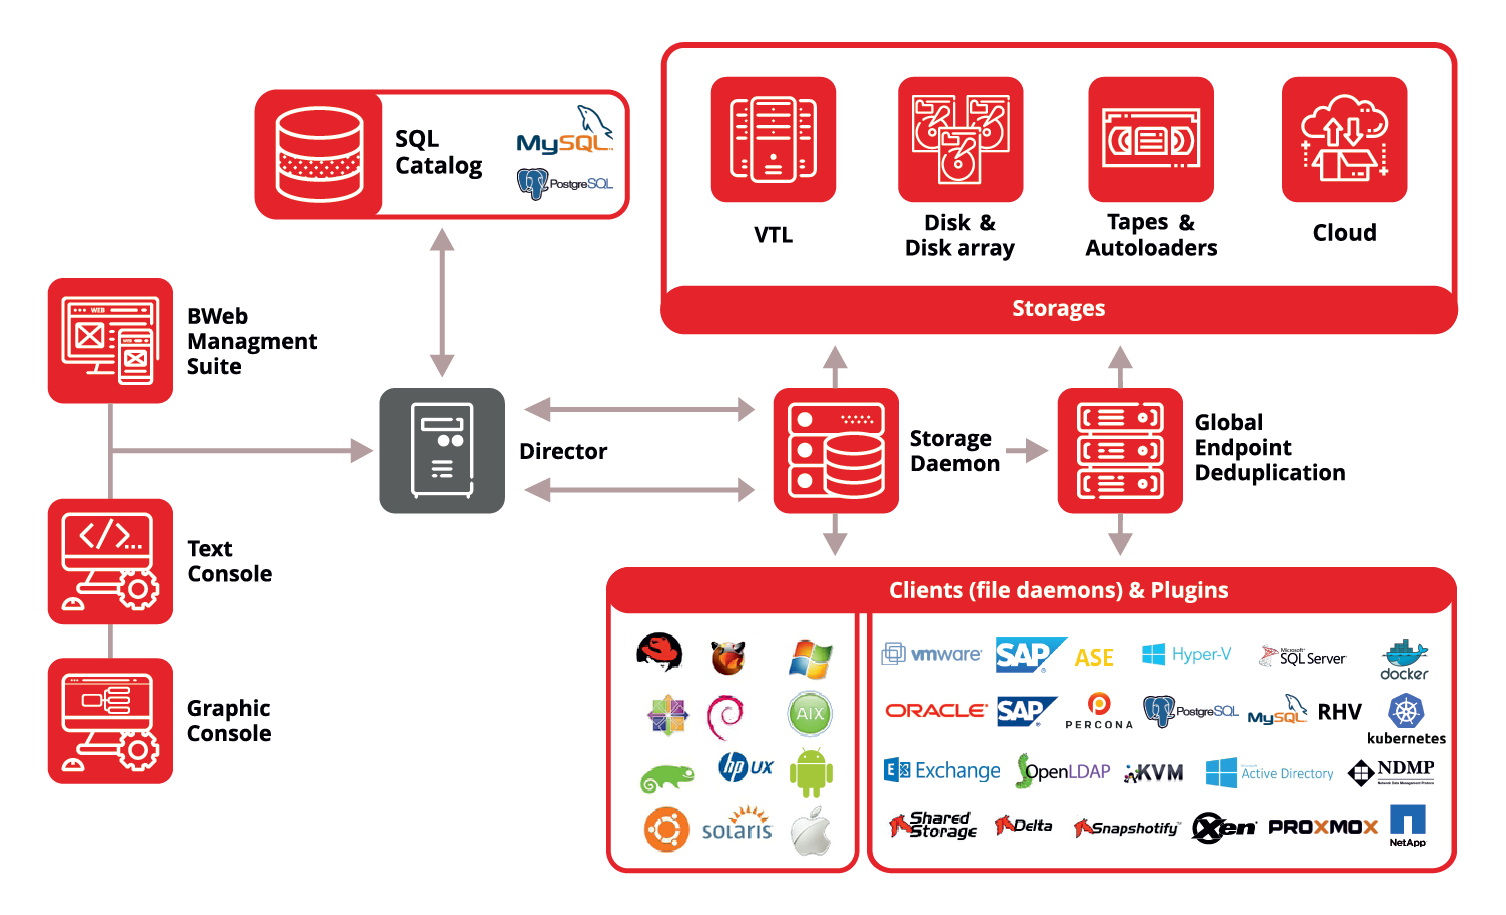
\includegraphics[height=80mm]{architecture.png}
  \end{center}  
 \note{
 Bacula est composé de 5 composants principaux :
\\~\\
\begin{description}
  \item[Director] il suppervise les opérations de sauvegarde, restauration, verification et archivage. C'est le composant principal et le point central des intéractions entre les composants.
  \item[Console] c'est l'interface qui permet aux utilisateurs de communiquer avec le composant Director. Il existe 2 versions :  un shell et une interface web.
  \item[Client (file daemon)] logiciel installé sur les machines clientes. Il est spécifique à l'OS sur lequel il est présent. Il sera chargé de transferer les données du client au storage et est aussi présent lors d'une opération de récupération.
  \item[Storage] composant responsable de l'écriture des sauvegardes sur les médias choisi: Par exemple sur des disques, les bandes et dans le cloud.
  \item[Catalog] stock les métadonnées pour toutres les activités de sauvegarde. 
  \item[-] est chargé de la maintenance des index de fichiers et des bases de données des volumes pour l'ensemble des sauvegardes. Il stock les informations sur les différentes sauvegardes réalisées ce qui rend la restauration et la gestion des volumes efficace.
\end{description}
}
\end{frame}

\begin{frame}{Architecture - Chiffrement}
 \begin{itemize}
  \item Chiffrement et signature des backups possible
  \item La master key doit être sauvegardée manuellement hors-site
  \item S'il y a perte de la master key, les backups sont perdus
 \end{itemize}
 \note{
 En ce qui concerne le chiffrement, Bacula permet de chiffrer et signer les données a sauvegardé. Les données sont chiffrées autant lors de la transmission que dans le backup lui-même.
\\~\\
\begin{itemize}
  \item Il faut tenir compte que seul le contenu des fichiers est chiffrés/signé alors que les métadonnées ne le sont pas (ça concerne par exemple : le nom du fichier, les permissions et le propriétaire du fichier).
  \item Attention, il est important d'avoir plusieurs sauvegardes de la master key utilisé pour le chiffrement car si on la perd, toutes les données chiffrées seront perdu.
  \item Communication via TLS =\> chiffrée (par ex Director - Console)
\end{itemize}
}

\end{frame}

\begin{frame}{Démonstration}
\end{frame}

\begin{frame}{CPU}
\begin{center}
  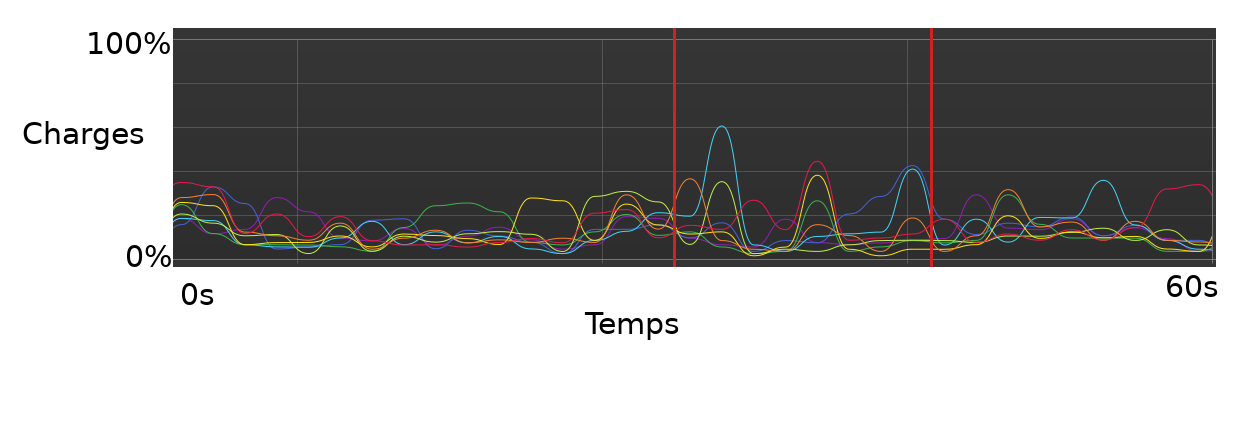
\includegraphics[height=50mm]{graphCPU}
\end{center}
\end{frame}

\begin{frame}{Coûts}
\begin{center}

\begin{itemize}
    \item 2 versions: Community Open Source et Entreprise
    \item La version Entreprise propose (entre autres) un expert qui permet d'apporter un support technique
    \item Dès 500\$ par mois sur devis pour la version Entreprise (abonnement Standard)
\end{itemize}

 \begin{tabular}{|l|ccccc|}
    \hline
    & Standard & Bronze & Silver & Gold & Platinum \\
    \hline
    \hline
    Nombre de clients & < 50 & < 200 & < 500 & < 2000 & < 5000 \\
    \hline
    Nombre de contacts & 1 & 2 & 3 & 5 & 5 \\
    \hline
    Assistance & Web & Web & Web et tél.& Web et tél. & Web et tél. \\
    \hline
    Nombre d'OS & 4 & toutes & toutes & toutes & toutes \\
    \hline
    Temps de réponse & 1j -- 4j & 6h -- 4j & 4h -- 2j & 1h -- 2j & 1h -- 2j \\ %heure/jour ouvrable
    du support &  & & & & \\
    \hline
    Formation & 0 & 0 & 0 & 0 & 1/an \\
    \hline
 \end{tabular}
\end{center}
\note{Il y a également l'option du temps de réponse du support qui dépendra donc du niveau de sévérité de la panne (il y a 4 niveaux différents, 4 étant la plus sévère). Il y a donc différentes intervalles de jours et d'heures par abonnement.
\\~\\
Je précise que ce sont seulement des jours ainsi que des heures ouvrables, donc le week-end n'est pas inclu. -\> donc quelque chose à prendre en compte
\\~\\
--\> au niveau des abonnements à prendre, tout dépend du besoin de l'entreprise et par exemple du besoin de disponibilité des données. Une entreprise qui possède un site web ou propose des services à des utilisateurs aura besoin d'un temps de réponse rapide, alors qu'une entreprise de recherche en informatique par exemple pourra accepter un temps de réponse plus large
\\~\\
Au niveau du coût total annuel de chaque abonnement, il est nécessaire de prendre contact avec Bacula afin de définir nos besoins spécifiques ainsi que notre projet de sauvegarde et restauration pour qu'ils fassent un devis. -\> Comme je l'ai dit avant, chaque entreprise a des besoins différents. Devis sur-mesure afin  de prendre l'abonnement qui convient le mieux
\\~\\
Il est également possible de télécharger une version d'essai de 1 mois afin de tester toutes les fonctionnalités ainsi que le support !! Mais on peut compter au minimum 500\$ par mois pour l'abonnement standard.
}
\end{frame}


\begin{frame}{Comparaison}
 \begin{center}
  \begin{tabular}{|l||c|c|c|c|c|c|c|c|c|c|}
    \hline
    & Coût & \rot{Open source ~} & Backups & \rot{Déduplication ~} & \rot{Chiffrement ~} & \rot{Compression ~} & \rot{Web interface} & \rot{Linux} & \rot{MacOS X} & \rot{Windows} \\
    \hline
    \hline
    Bacula & \makecell{Gratuit\\Payant} & \cellcolor{green!50} & \makecell{Full\\ Incrémentaux\\ Différentiels} & \cellcolor{green!50} & \cellcolor{green!50} & \cellcolor{green!50} & \cellcolor{green!50} & \cellcolor{green!50} & \cellcolor{green!50} & \cellcolor{green!50} \\
    \hline
    BorgBackup & \makecell{Gratuit\\Payant} & \cellcolor{green!50} & \makecell{Full\\ Incrémentaux\\ Différentiels} & \cellcolor{green!50} & \cellcolor{green!50} & \cellcolor{green!50} & \cellcolor{orange!50} & \cellcolor{green!50} & \cellcolor{green!50} & \cellcolor{red!50} \\
    \hline
    Bup & Gratuit & \cellcolor{green!50} & Incrémentaux & \cellcolor{green!50} & \cellcolor{red!50} & \cellcolor{green!50} & \cellcolor{green!50} & \cellcolor{green!50} & \cellcolor{green!50} & 
    \cellcolor{red!50} \\
    \hline
    Duplicati & Gratuit & \cellcolor{green!50} & \makecell{Full\\ Incrémentaux} & \cellcolor{green!50} & \cellcolor{green!50} & \cellcolor{green!50} & \cellcolor{green!50} & \cellcolor{green!50} & \cellcolor{green!50} & \cellcolor{green!50} \\
    \hline
    Rsync & Gratuit & \cellcolor{green!50} & Incrémentaux & \cellcolor{red!50} & \cellcolor{red!50} & \cellcolor{red!50} & \cellcolor{red!50} & \cellcolor{green!50} & \cellcolor{green!50} & \cellcolor{green!50}  \\
    \hline
 \end{tabular}
 \begin{tablenotes}
 \scriptsize 
  \fcolorbox{black}{green!50}{\rule{0pt}{4pt}\rule{4pt}{0pt}}\quad Oui \fcolorbox{black}{red!50}{\rule{0pt}{4pt}\rule{4pt}{0pt}}\quad Non
  \fcolorbox{black}{orange!50}{\rule{0pt}{4pt}\rule{4pt}{0pt}}\quad En développement
    \end{tablenotes}
 \end{center}
 \note{Les outils que je vais comparer avec Bacula c'est BorgBackup, Bup, Duplicati ainsi que rsync.
\\~\\
Bacula propose deux versions de son logiciel, une gratuite qui est open source et une autre payante. BorgBackup propose également ces deux options. Sinon tous les outils propose une version gratuite et open-source.
\\~\\
Bacula permet d'effectuer des backups de 3 manières différentes, full/incrémental/différentiel, BorgBackup le permet aussi. Sinon l'outil Duplicati propose le backup différentiel en moins.
\\~\\
La plupart des outils comparés peuvent être utilisés avec les systèmes d'exploitation Linux, MacOS et Windows. Il y a juste BorgBackup et Bup qui ne supporte pas Windows.
\\~\\
-\> on constate finalement que Bacula est un outil complet qui est assez flexible. Mais BorgBackup peut également être une alternative possible, mais seulement si on n'utilise pas Windows.
 }
\end{frame}

\begin{frame}{Avantages / inconvénients}
    \begin{center}\small
     \begin{tabular}{|l|l|}
     \hline
      \textbf{Avantages} & \textbf{Inconvénients} \\
     \hline
     \hline
        Interface utilisateur graphique & Prise en main complexe (fichiers \\ 
                                        & de configuration) \\
     \hline
     Cross-platform & Pas de scan de virus \\
     \hline
     Automatisation \& planification des tâches & Configuration nécessaire au backup \\ 
                                                & des appareils mobiles\\
     \hline
     Sauvegarde continue (CDP) & \\
     \hline
     Toujours maintenu (dernière update : juin 2021) & \\
     \hline
     Sauvegarde Cloud \& hors-site & \\
     \hline
     Charge réseau \& CPU modulables & \\
     \hline
     Déduplication des données & \\
     \hline
     Support d'environnements virtuels & \\
     \hline
     Large documentation et en plusieurs langues & \\
     \hline
     \end{tabular}

    \end{center}
\note{
Bacula n'est \textbf{pas prévu pour effectuer des sauvegardes d'appareils connectés sporadiquement} mais pour des serveurs avec des adresses IP fixes. Le problème intervient quand l'appareil n'est pas connecté sur le réseau mais que le Director Daemon le cherche malgré tout. Il est tout de même possible de configurer Bacula pour cette situation spécifique avec un script, mais cela ajoute un peu de complexité. 
\\~\\
Il est possible de \textbf{modifier la priorité des processus de sauvegarde pour soulager le CPU}, ainsi que de moduler les types de backup et leur fréquence pour ne pas trop empiéter sur le réseau. 
\\~\\
La \textbf{déduplication élimine les copies excessives} de données et réduit considérablement les besoins en capacité de stockage. Elle s'effectue en arrière plan et ne ralentit donc pas la sauvegarde. Bacula utilise également un mécanisme de compression pour réduire la taille des fichiers et accélérer les processus. Cette déduplication des données permet d'alléger la charge réseau engendrée. 
\\~\\
Prise en main (conf) / Scan virus / config mobile 
\\~\\ 
GUI / Cross / Automatisation / Cdp / Mantenu / Cloud - hors-site / réseau CPU / Dédup. / Env. virtuelle / Doc
}
\end{frame}

\begin{frame}{Conclusion}
 \begin{itemize}
  \item Sauvegarde jusqu'à 1x par heure - RPO très faible
  \item Automatisation et planification possibles
  \item Economie de temps, d'argent, de stress
 \end{itemize}
 \note{
 Bacula est très flexible et les sauvegardes peuvent être planifiées au bon vouloir de l'administrateur, cela signifie que des backups peuvent être effectués jusqu'à une fois par heure. Cela nous donne un RPO (Recovery Point Objective) très faible. Ce RPO dépend de la manière dont Bacula est configuré. 
\\~\\
Le RPO très faible et l'automatisation possible des sauvegardes engendrent une réelle économie pour l'entreprise, on économise le temps des employés et leur travail qu'on ne risque pas de trop perdre.
}
\end{frame}

\begin{frame}{Questions ?}
  \begin{center}
    
\includegraphics[height=60mm]{bat_kitty.jpg}
  \end{center}  
\end{frame}


\end{document}
